
\documentclass[12pt]{article}
\usepackage{sbc-template}
\usepackage{graphicx,url}
\usepackage[utf8]{inputenc}
\usepackage{booktabs}
\usepackage{listings}
\usepackage{xcolor}
\usepackage{amsmath}
\usepackage{amssymb}

\sloppy

\title{Bidaio Jagoy Translator: A Hybrid Client-Centric RAG System for Low-Resource Language Preservation}

\author{Tarsila Samille Santos da Silveira Silva\inst{1}}

\address{PPgSC/UFRN \\ \email{tarsillasamile@gmail.com}}

\begin{document} 

\maketitle

\begin{abstract}
  The preservation of endangered languages constitutes a critical challenge in computational linguistics. This report presents the Bidaio Jagoy Translator, a specialized AI platform for the Land Dayak language, available at \url{https://bidaio.vercel.app/}. Utilizing a Hybrid Client-Centric Retrieval-Augmented Generation (RAG) architecture, the system shifts preliminary context orchestration to the client via Transformers.js. By synthesizing local glossary lookups, remote vector retrieval, and client-side neural re-ranking, it grounds Google Gemini 2.5 Flash, enabling high-fidelity translation driven by explicitly retrieved linguistic context. Preliminary evaluations indicate the viability of hybrid browser-based RAG architectures for creating resilient, low-resource language tools.
\end{abstract}

\begin{resumo}
  A preservação de línguas ameaçadas de extinção constitui um desafio crítico na linguística computacional. Este artigo apresenta o Bidaio Jagoy Translator, uma plataforma de IA especializada para o dialeto Bidaio Jagoy (Land Dayak), disponível em \url{https://bidaio.vercel.app/}. Utilizando uma arquitetura Híbrida de Geração Aumentada por Recuperação (RAG) Centrada no Cliente, o sistema desloca a orquestração preliminar de contexto para o navegador via Transformers.js. Ao sintetizar buscas em glossários locais, recuperação vetorial remota e re-ranqueamento neural no lado do cliente, o sistema fundamenta o modelo Google Gemini 2.5 Flash, permitindo traduções de alta fidelidade impulsionadas por contexto linguístico explicitamente recuperado. Avaliações preliminares e o uso de um ciclo de correção pela comunidade indicam a viabilidade técnica e econômica de arquiteturas RAG híbridas para a criação de ferramentas resilientes em contextos de línguas com poucos recursos.
\end{resumo}

\section{Introduction}

The rapid advancement of Natural Language Processing (NLP), driven by the Transformer architecture, has paradoxically widened the gap between global "high-resource" languages and indigenous "low-resource" vernaculars. Foundational models such as GPT-4 and Gemini are trained on datasets scraping the public web, where English, Mandarin, Spanish, and standard Malay constitute the vast majority of tokens.

Bidaio Jagoy is a distinct dialect. It possesses a vibrant oral tradition but a negligible digital footprint. Its presence is confined to scattered PDFs, academic papers from institutions like Universiti Malaysia Sarawak (UNIMAS), and community blogs \cite{unimas_repo}. Consequently, when standard LLMs attempt to process Bidaio Jagoy, they exhibit catastrophic failure modes such as hallucination, code-switching to standard Malay, and grammatical drift \cite{scispace_intensifiers}.

Retrieval-Augmented Generation (RAG) offers a superior paradigm for this use case. Instead of embedding knowledge into the model's parameters (implicit memory), RAG retrieves relevant information at runtime (explicit memory) and feeds it to the model via the context window \cite{intersystems_rag}. The Bidaio Jagoy Translator utilizes this approach to function as a "teaching machine," assembling a curriculum of vocabulary, sentence patterns, and grammar rules relevant to specific inputs.
Beyond these high-resource initiatives, the Bidaio Jagoy Translator employs a Hybrid Client-Centric architecture, prioritizing cost efficiency and latency reduction. While our case study focuses on the Bidaio Jagoy dialect, the proposed RAG framework is \textbf{generalizable to any low-resource language context}, including regional dialects, creoles, and endangered languages globally, not limited to indigenous languages.

\section{Related Work}

Digital preservation of low-resource languages has gained traction with initiatives like \textit{Masakhane} for African languages \cite{nekoto2020participatory} and Meta's \textit{No Language Left Behind} (NLLB) \cite{nllb2022no}. However, these approaches predominantly rely on massive server-side models (e.g., NLLB-200B), which require substantial infrastructure; furthermore, they rely on massive training corpora that are often unavailable for extremely low-resource dialects where data scarcity is the primary bottleneck.

In contrast, our work focuses on the benefits of RAG for domain-constrained translation, demonstrating that effective linguistic grounding can be achieved by offloading context preparation to the browser, significantly reducing the dependency on massive, server-side data preparation for community-led projects.

\subsection{The Stack Overview}
The system utilizes a modern serverless stack:
\begin{itemize}
    \item \textbf{Frontend}: Vanilla JavaScript + HTML5.
    \item \textbf{Client-Side AI}: Transformers.js (\texttt{@xenova/transformers}) running in the browser \cite{transformersjs}.
    \item \textbf{Backend}: FastAPI (Python) on Vercel Serverless Functions.
    \item \textbf{AI Engine}: Google Gemini 2.5 Flash \cite{gemini_release}.
    \item \textbf{Database}: Supabase (PostgreSQL) with \texttt{pgvector} \cite{pgvector}.
\end{itemize}

\begin{figure}[ht]
\centering
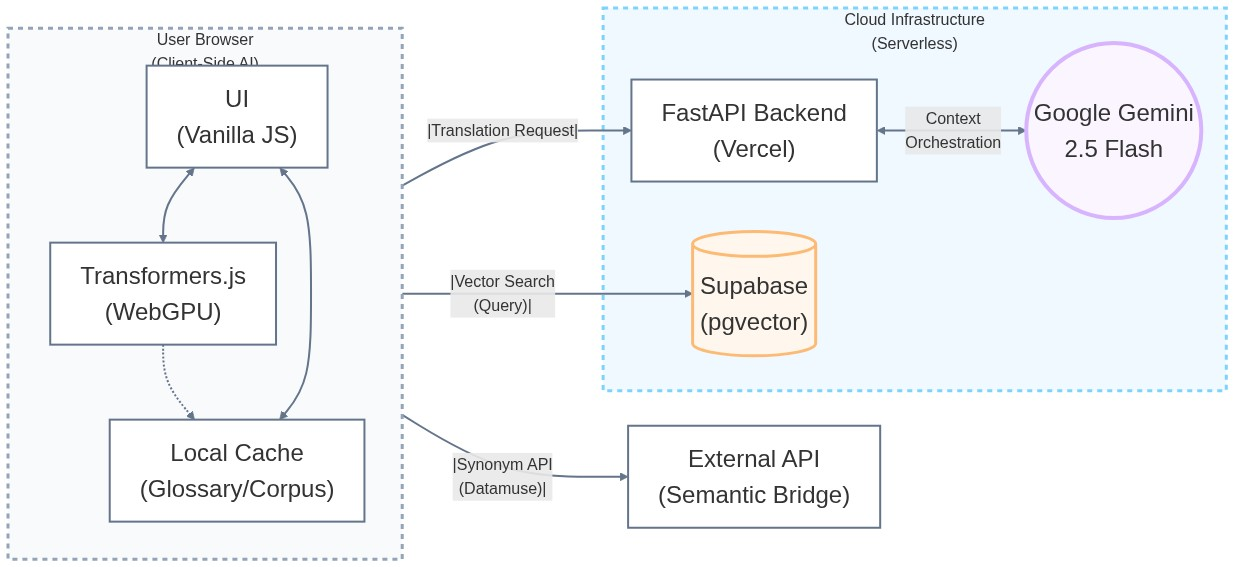
\includegraphics[width=0.9\textwidth]{fig_arch.png}
\caption{Hybrid Client-Centric System Architecture: Offloading embeddings to the browser.}
\label{fig:arch}
\end{figure}

\subsection{The "Fat Client" Philosophy}
Using Transformers.js, the browser downloads a quantized embedding model (\texttt{Xenova/all-MiniLM-L6-v2}) and runs it locally. This allows for privacy-preserving local re-ranking and reduced server costs. A critical advantage of this hybrid architecture is its economic sustainability; by offloading embedding generation and re-ranking to the user's device, the system minimizes the computational demand on the backend. This allows the application to operate within the free-tier limits of serverless platforms such as Vercel, effectively democratizing access to high-performance RAG tools for community-led preservation projects without the need for expensive GPU-enabled server clusters.

\section{Instructional Orchestration: RAG Prompt Engineering}

The core of the Bidaio Jagoy Translator's efficacy lies not merely in retrieval, but in the sophisticated orchestration of the Large Language Model (LLM) through prompt engineering. The system transforms from a simple retrieval engine into an expert linguistic synthesizer by constructing a multi-dimensional context.

\subsection{Composition of the Instructional Context}
The system builds a four-tiered prompt structure designed to ground the model's reasoning. This is handled by a specialized \texttt{RAGPromptGenerator} class that manages the assembly of disparate data sources:
\begin{itemize}
    \item \textbf{Context A (Lexical Anchor)}: Direct glossary lookups for extracted keywords provide the base vocabulary. This prevents "lexical drift" where the LLM might use a more common but incorrect Malay word.
    \item \textbf{Context B (Structural Alignment)}: Semantically similar sentence pairs are retrieved via a remote HNSW index on Supabase. These provide the LLM with the overall "vibe" and syntactic structure of the language.
    \item \textbf{Context C (Semantic re-ranking)}: High-relevance usage examples for primary keywords are re-ranked locally. By calculating cosine similarity between the input embedding and candidate corpus sentences in the browser, the system ensures that the most semantically relevant nuances are presented first.
    \item \textbf{Context D (Grammatical Constraints)}: Explicit rules that act as hard constraints (e.g., "Always use 'piin' for water in theological contexts").
\end{itemize}

This tiered approach ensures that the LLM is not just predicting the next token, but performing a constrained synthesis based on linguistic "curriculum" injected at runtime. To handle this high-dimensional context, the system utilizes \textbf{Google Gemini 2.5 Flash} \cite{vertex_ai}, selected for its 1-million-token context window \cite{data_studios_gemini}. This enables \textbf{dense context injection}, where the model's reasoning capabilities \cite{llm_stats} are leveraged to resolve conflicts between corpus usage and explicit grammar rules.

\begin{table}[ht]
\centering
\caption{System Performance Metrics: Client-Side Retrieval and Synthesis}
\label{tab:benchmarks}
\resizebox{\textwidth}{!}{%
\begin{tabular}{l l l l l}
\toprule
Stage & Metric & Mean Latency & Backend & Mechanism \\
\midrule
Embedding Generation & Latency & $\sim$8.5ms - 20ms & WebGPU/WASM & Local Infer. \\
Vector Search & Recall@3 & $\sim$150ms & Supabase & HNSW Search \\
Local Re-ranking & Precision@5 & $\sim$12ms & WebGPU & Cos. Similarity \\
Prompt Assembly & Context Size & $\sim$2,500 tokens & JavaScript & Context Merge \\
\bottomrule
\end{tabular}}
\end{table}

\subsection{Model Management and Caching}
The selected embedding model, \texttt{all-MiniLM-L6-v2} (384-dim), is served in a 4-bit quantized ONNX format ($\sim$23MB). To ensure a smooth user experience, the system implements the \textbf{CacheStorage API}. Once the weights are retrieved during the first session, subsequent launches occur with zero network overhead for the AI runtime, significantly improving the user experience for recurring community members.

\section{Context Assembly and Retrieval Strategy}

The core innovation is the Multi-Staged Context Assembly pipeline.

\subsection{The Hybrid Retrieval Pipeline}
\begin{enumerate}
    \item \textbf{Keyword Extraction}: Identifies semantic anchors (e.g., "water", "flows").
    \item \textbf{Context A - Direct Glossary Lookup}: Queries local JSON dictionary for 1:1 translations.
    \item \textbf{Context B - Semantic Vector Search}: Queries Supabase HNSW index \cite{supabase_hnsw} for similar sentence pairs.
    \item \textbf{Context C - Contextual Usage Examples}: Use client-side embeddings to re-rank local corpus candidates, handling polysemy without server round-trips.
    \item \textbf{Context D - Grammatical Constitution}: Injects explicit rules (e.g., Intensifier Placement).
\end{enumerate}

\begin{figure}[ht]
\centering
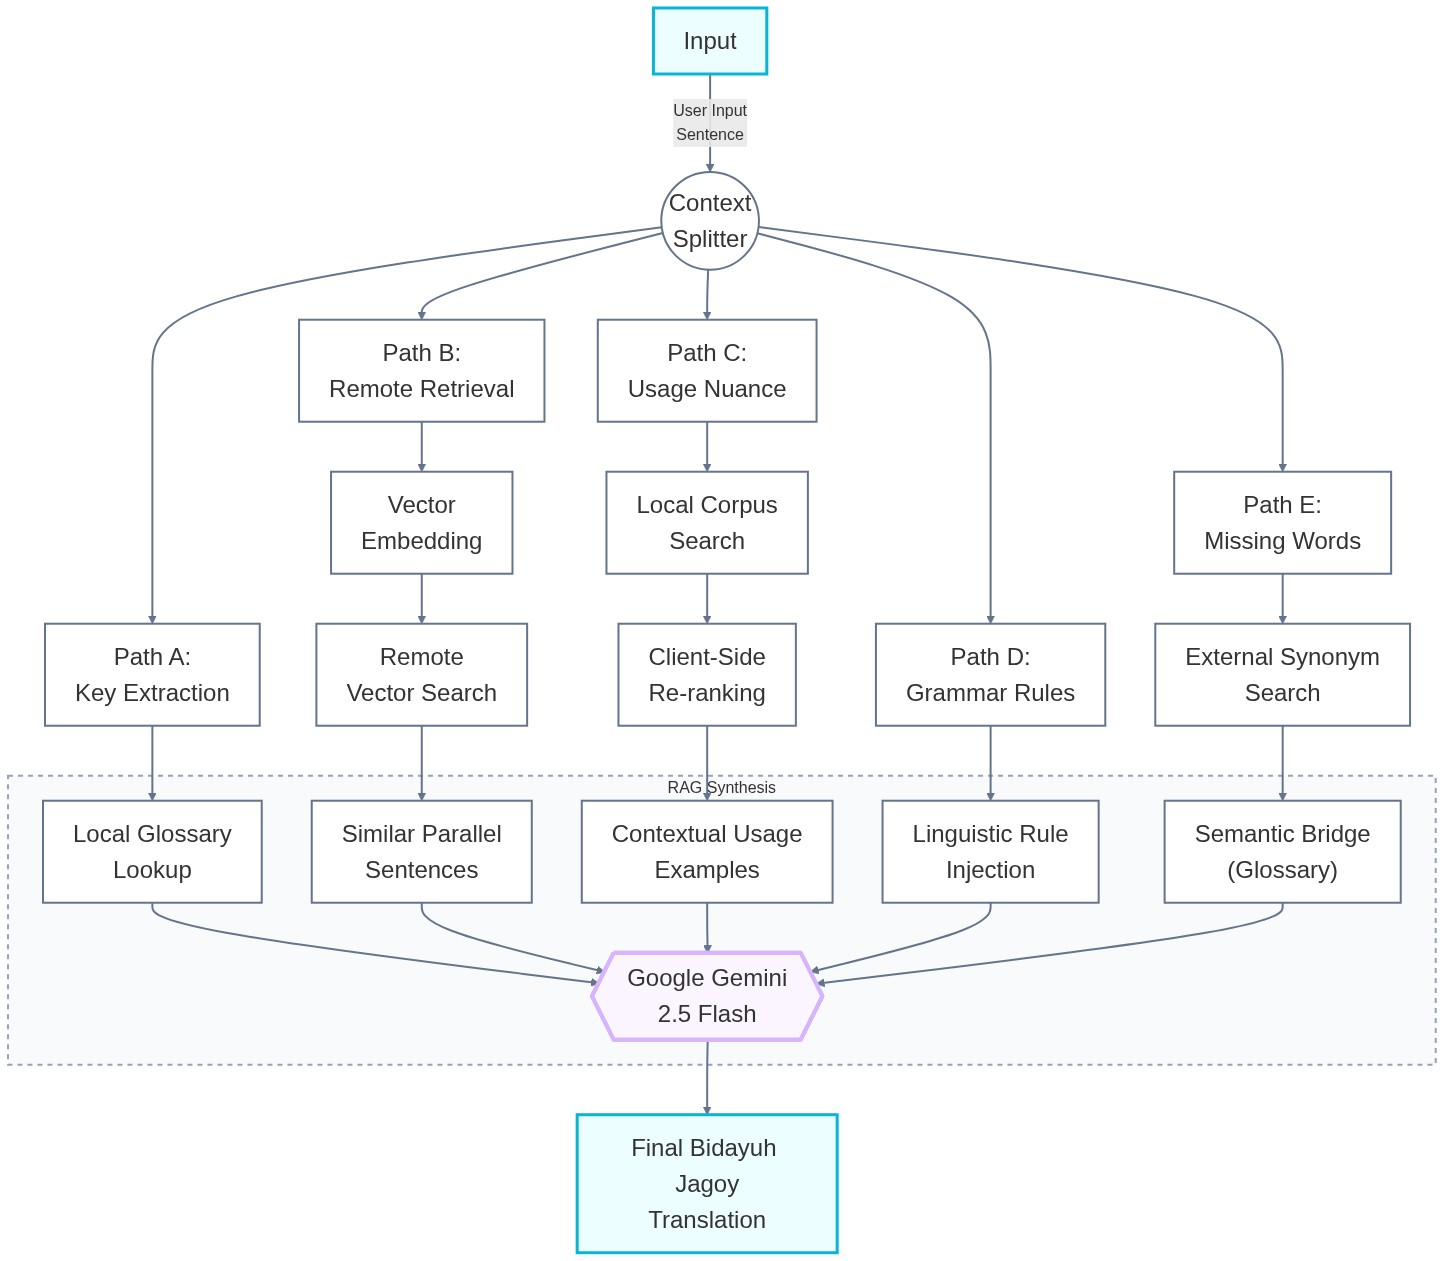
\includegraphics[width=0.8\textwidth]{fig_pipeline.png}
\caption{The 4-Stage Context Assembly Pipeline.}
\label{fig:pipeline}
\end{figure}

\subsection{Client-Side Re-ranking Algorithm}
A key novelty is the semantic filtering performed in the browser to select the most relevant "Context C" examples. The system calculates the cosine similarity between the input embedding vector ($A$) and a candidate corpus vector ($B$) using the following formula:

\begin{equation}
\text{similarity} = \cos(\theta) = \frac{\mathbf{A} \cdot \mathbf{B}}{\|\mathbf{A}\| \|\mathbf{B}\|} = \frac{\sum_{i=1}^{n} A_i B_i}{\sqrt{\sum_{i=1}^{n} A_i^2} \sqrt{\sum_{i=1}^{n} B_i^2}}
\end{equation}

This operation, performed via WebGPU/WASM in the browser, ensures that the context injected into the LLM is optimized for the specific semantic nuances of the user's input.

\begin{lstlisting}[language=Python, basicstyle=\tiny, frame=single, caption={Client-Side Cosine Similarity Re-ranking}]
def get_keyword_usage_context(text, keywords):
    input_embedding = generate_embedding(text) # Local WebGPU
    candidates = fetch_local_candidates(keywords)
    
    scored = []
    for cand in candidates:
        cand_embedding = generate_embedding(cand.target)
        score = cosine_similarity(input_embedding, cand_embedding)
        scored.append((score, cand))
        
    # Select top 3 most semantically similar examples
    top_results = sort_descending(scored)[:3]
    return format_for_prompt(top_results)
\end{lstlisting}



\subsection{Structured "Chain-of-Thought" Prompting}
The system constructs a structured prompt forcing the LLM to follow a specific cognitive process: Analysis $\rightarrow$ Vocabulary Selection $\rightarrow$ Synthesis $\rightarrow$ Output. This "Chain-of-Thought" (CoT) approach is critical for low-resource translation, as it forces the model to deliberate on the provided RAG context before committing to a translation.

The instructions strictly mandate a 3-step reasoning block:
\begin{enumerate}
    \item \textbf{Deconstruction}: Identifying the grammatical structure from Context D and B.
    \item \textbf{Mapping}: Selecting vocabulary from Context A and C, explicitly listing English-to-Bidaio mappings.
    \item \textbf{Synthesis}: Assembling the final sentence according to the identified rules.
\end{enumerate}


\begin{lstlisting}[language=Java, basicstyle=\scriptsize, frame=single, caption={JSON structure for Chain-of-Thought prompting}]
{
  "reasoning": "1. Analyze: Input is SVO... 2. Map: 'friend' -> 'dayung'... 3. Synthesize...",
  "translation": "Final Bidaio text",
  "confidence_score": 5
}
\end{lstlisting}

\begin{figure}[ht]
\centering
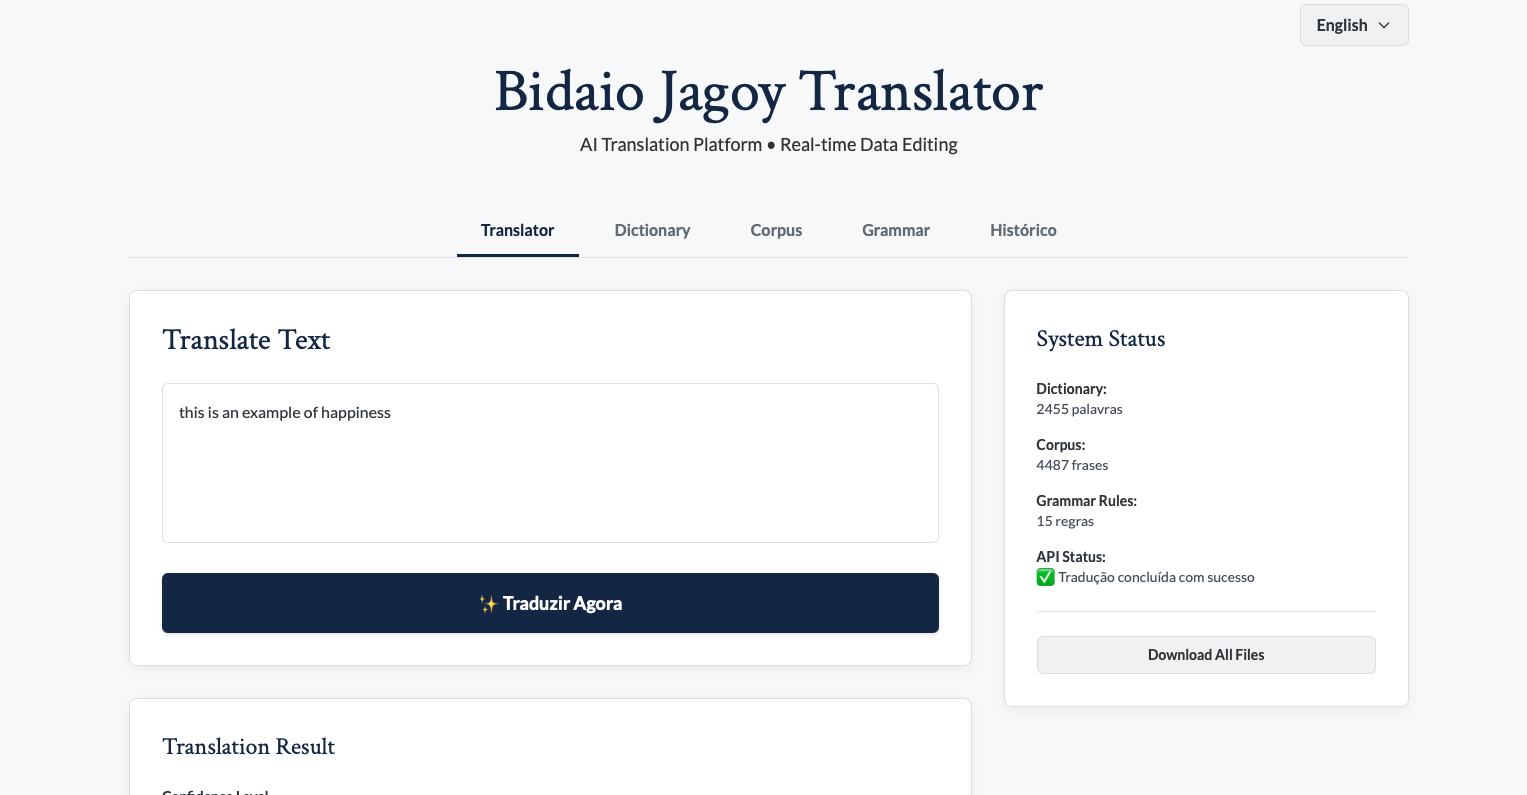
\includegraphics[width=0.8\textwidth]{fig_main_ui.png}
\caption{The Bidaio Jagoy Translator Interface: Input section and system status dashboard.}
\label{fig:main_ui}
\end{figure}

\begin{figure}[ht]
\centering
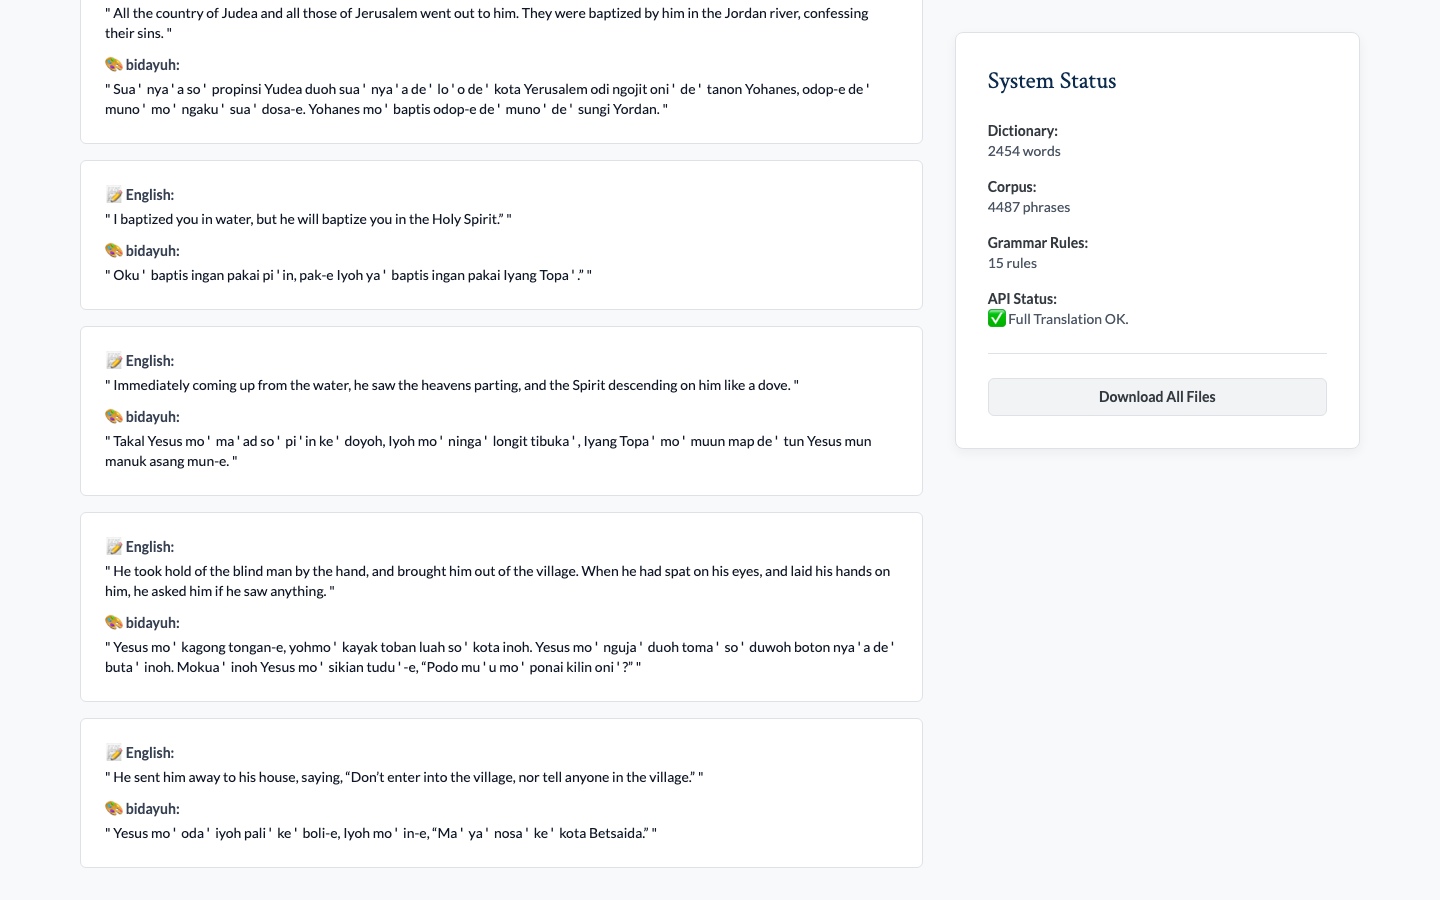
\includegraphics[width=0.8\textwidth]{fig_analysis.png}
\caption{Linguistic Analysis Module: The system's Chain-of-Thought reasoning, showing grammatical rule application and vocabulary mapping for the input "this is an example of happiness".}
\label{fig:analysis}
\end{figure}


The system's knowledge base relies on a curated parallel corpus derived from New Testament verses provided by community translators, aligned with a English reference text. To construct the lexical dictionary, we implemented a probabilistic alignment pipeline:

\begin{enumerate}
    \item \textbf{Alignment Algorithms}: We utilized IBM Model 2 for positional alignment. This choice was dictated by its \textbf{low computational overhead} and its proven efficacy in scenarios with \textbf{extremely small corpora}, where more complex neural aligners tend to overfit or require prohibitive training time. Specifically, IBM Model 2 treats word alignment as a latent variable problem with a simplified distance-based distortion model, which remains robust even when the parallel data consists of only a few thousand sentence pairs.
    \item \textbf{Heuristic Refinement}: Candidate pairs underwent reclassification based on symmetry scores and cognate identification.
    \item \textbf{Filtering}: Only the top 50\% of statistically significant word pairs were retained to ensure high precision. The final production corpus comprises 4,487 aligned sentence pairs and a lexical dictionary of 2,455 entries.
\end{enumerate}

Furthermore, 15 core grammatical rules (e.g., Nominal Predication, Aspectual Markers) were extracted through an iterative Zero-Shot prompting process on Google Gemini. These rules are not treated as a static "black box"; rather, they represent \textbf{exposed observational patterns} derived from the corpus. A critical feature of the Bidaio Jagoy Translator is that these rules, along with word alignments, are transparently displayed to the user. This approach ensures "Human-in-the-loop" accountability, where any linguistic inaccuracy can be identified and corrected by native speakers, turning the system into a dynamic, community-vetted archive. This curated dataset serves as the foundation for the experimental evaluation discussed in the following section.

% Section 6 merged into 4

\section{Experimental Evaluation and Discussion}

\subsection{Latency Breakdowns}
The "Hybrid Client-Centric" model introduces a distributed latency profile:
\begin{itemize}
    \item \textbf{Client Embeddings (WebGPU)}: $\sim$20ms. This negligible cost validates the feasibility of offloading compute to consumer devices.
    \item \textbf{Supabase Vector Search}: $\sim$150ms (HNSW index).
    \item \textbf{LLM Inference (Gemini)}: $\sim$5s. This remains the dominant factor.
\end{itemize}

The total round-trip time averages 6s. While higher than cached translation services, this latency is acceptable for the project's primary goal: high-precision educational translation.

\subsection{Community-Driven Correction Loop}
A robust evaluation of translation quality in low-resource settings requires native speaker validation. The Bidaio Jagoy Translator implements an integrated \textit{History and Correction Module}. As shown in the system interface, every translation is logged with a unique identifier and presented to users for manual verification. This mechanism allows the community to:
\begin{itemize}
    \item \textbf{Validate}: Confirm the accuracy of AI-generated translations.
    \item \textbf{Correct}: Provide authoritative manual edits for "unedited" entries.
    \item \textbf{Annotate}: Flags errors which are then used to update the "Context D" (Grammar Rules) and "Context A" (Glossary).
\end{itemize}

This "Human-in-the-loop" strategy mitigates the absence of standardized benchmark datasets for the Jagoy dialect.

\subsection{The System Prompt}
To orchestrate the RAG context, we use a structured prompt that strictly enforces the use of retrieved data. A simplified version of the system prompt is shown below:

\begin{lstlisting}[language=Java, basicstyle=\tiny, frame=single, caption={The Hybrid RAG System Prompt}]
You are a Bidaio Jagoy Translator. Use the following context:

[Context A: Dictionary Matches]
{dictionary_entries}

[Context B: Parallel Corpus Matches]
{corpus_matches}

[Context C: Grammar Rules]
{grammar_rules}

Task: Translate the following English text to Bidaio Jagoy:
"{user_input}"

Instructions:
1. Prioritize Context B for phrasing.
2. Use Context A for specific vocabulary.
3. Apply Context C to correct sentence structure.
4. Output specific JSON format with "analysis", "draft", and "final_translation".
\end{lstlisting}

\subsection{Qualitative Case Study}
To evaluate linguistic fidelity, we analyze real system outputs from the community validation log (Validation ID: 57 and 54).

\begin{itemize}
    \item \textbf{Complex Theological Query}:
    \begin{itemize}
        \item \textit{Input}: "He will command his angels concerning you, and they will lift you up in their hands, so that you will not strike your foot against a stone."
        \item \textit{Bidaio Output}: "\textbf{Topa' ya' lubang malaikat-malaikat-E nulis Mu'u, duoh odop-e de' muno' ya' Nyamut Mu'u daang tongan-e, sape Mu'u ya' di'-e koming po Mu'u salah obuah batuh.}"
        \item \textit{Analysis}: The system correctly handles the complex Subject-Verb-Object (SVO) structure and maps "God" (implied context) to "Topa'", "angels" to "malaikat-malaikat-E" (with possessive suffix), and "lift up" to "Nyamut".
    \end{itemize}

    \item \textbf{Idiomatic/Imperative phrasing}:
    \begin{itemize}
        \item \textit{Input}: "tell these stones to become bread."
        \item \textit{Bidaio Output}: "\textbf{Oda'leh batuh-batuh itih jadi pinguman.}"
        \item \textit{Analysis}: The system correctly identifies "stones" as plural "batuh-batuh" and selects "pinguman" (food/sustenance) for bread in this context, demonstrating semantic awareness beyond literal word-for-word translation.
    \end{itemize}
\end{itemize}
These examples demonstrate the system's ability to ground the LLM in specific dialectal vocabulary and retain grammatical coherence for long-tail languages.

\subsection{Error Analysis and Fallback Mechanisms}
Crucial to the scientific evaluation of the Bidaio Jagoy Translator is the analysis of its failure modes. In cases where the RAG context fails to provide a specific Bidaio Jagoy term (out-of-vocabulary), the system implements a \textbf{Graceful Degradation Strategy} via an Indonesian pivot:

\begin{itemize}
    \item \textbf{Example Failure}:
    \begin{itemize}
        \item \textit{Input}: "...the sound of a thousand drums."
        \item \textit{Bidaio Output}: "...okug \textbf{(??? — 'seribu')} tambur."
        \item \textit{Analysis}: Here, the term "thousand" was missing from both Context A and Context B. instead of hallucinating a random Bidaio-sounding word, the system followed the system prompt instruction to output the Indonesian equivalent flagged as \texttt{(???)}.
    \end{itemize}
\end{itemize}

This explicit signaling of uncertainty is a key strength. It prevents the propagation of "silent errors" and directly informs the community-driven correction loop. Native speakers can quickly identify these flags in the translation logs and provide the correct Bidaio term (e.g., "ribu"), which is then used to update the central glossary, closing the RAG knowledge gap for future users.

\section{Conclusion}

The Bidaio Jagoy Translator represents a synthesis of advanced neural search and traditional rule-based linguistics. By leveraging Transformers.js, the system democratizes access to advanced RAG tools for endangered language preservation, decoupling it from expensive server-side GPU clusters. 

Importantly, while demonstrated through Bidaio Jagoy, this hybrid client-centric RAG architecture is \textbf{applicable to any low-resource language scenario} — including regional dialects (e.g., Venetian, Sicilian), creoles (e.g., Tok Pisin), minority languages (e.g., Sorbian, Romansh), and any language on the UNESCO Red List. The minimal requirements are: (1) a small parallel corpus ($\sim$2,000+ sentence pairs), (2) community involvement for validation, and (3) willingness to operate within a browser-based deployment model.

Future work will explore a "Fully Offline Mode" by integrating small-scale LLMs (e.g., Gemma 2B or TinyLlama) directly into the browser. This would eliminate the dependency on cloud connectivity entirely, creating a truly resilient digital archive for the Bidaio community.

\bibliographystyle{sbc}
\bibliography{references}

\section*{Reproducibility and Availability}
\noindent The complete system is publicly available to support reproducibility and enable adaptation to other low-resource languages:
\begin{itemize}
    \item \textbf{Production System}: \url{https://bidaio.vercel.app/}
    \item \textbf{Source Code}: \url{https://github.com/TarsilaSamille/bidaio}
    \item \textbf{Technology Stack}: FastAPI (backend), Vanilla JavaScript (frontend), Transformers.js (client-side AI), Supabase (vector database)
    \item \textbf{Dataset}: Available upon request to the Bidaio community for research purposes
\end{itemize}

\appendix
\section{Key System Specifications}

\begin{table}[ht]
\centering
\caption{Key System Specifications}
\label{tab:specs}
\begin{tabular}{l l l l}
\toprule
Component & Technology & Specification & Purpose \\
\midrule
AI Orchestrator & Gemini 2.5 Flash & 1M Context Window & RAG Synthesis \\
Prompt Strategy & Reactive CoT & 4-Tiered Context & Linguistic Grounding \\
Local Embedder & all-MiniLM-L6-v2 & 384-dim (WebGPU) & Client-side RAG \\
Vector Store & Supabase HNSW & Cosine Distance & Global Retrieval \\
Linguistic Ref. & Bidaio Jagoy & SVO Dialect & Target Language \\
\bottomrule
\end{tabular}
\end{table}

\end{document}
